\documentclass{llncs}
\usepackage{graphicx}
\usepackage{color}
\usepackage{enumitem}
\usepackage{hyperref}
\usepackage{dirtytalk}
\usepackage[utf8]{inputenc}
\hypersetup{
    colorlinks=true,
    linkcolor=blue,
    filecolor=magenta,      
    urlcolor=cyan,
}
%%%%%%%%%%%%%%%%%%%%%%%%%%%%%%%%%%%%%%%%%%%%%%%%%%%%%%%%%%%%%%%%%%%%%%%%%%
\usepackage{todonotes} % use this to see the comments
%\usepackage[textsize=tiny]{todonotes} % use this to see SMALL : ) comments
%\usepackage[disable]{todonotes} % use this to hide all comments
%%%%%%%%%%%%%%%%%%%%%%%%%%%%%%%%%%%%%%%%%%%%%%%%%%%%%%%%%%%%%%%%%%%%%%%%%%


\newcommand{\todoinline}[1]{
    \todo[inline]{#1}
}
\newcommand{\todoiteminline}[3]{
    \todoitemtemplate{#1}{#2}{#3}{inline}{red}
}

\newcommand{\todoproofread}[3]{
    \todoitemtemplate{#1}{#2}{Please proof read above section; #3}{inline}{yellow}
}
\definecolor{mygreen}{HTML}{00CC00}
\newcommand{\todoproofreadDone}[3]{
    \todoitemtemplate{#1}{#2}{Please proof reading above section, done; #3}{inline}{mygreen}
}
\newcommand{\todoproofreaddone}[3]{
    \todoproofreadDone{#1}{#2}{#3}
}

\newcommand{\todoitemtemplate}[5]{%
% \index[MYTODO]{#2}
\todo[#4,color=#5,caption=X]{{#1}{ \textbf{{\tiny{for}} #2}:}{#3}}%
}

\newcommand{\todoiteminlinedone}[3]{
    \todoiteminlineDone{#1}{#2}{#3}
}
\newcommand{\todoiteminlineDone}[3]{
    \todoitemtemplate{{\commentsDoneFont{#1}}}{{\commentsDoneFont{#2}}}{{\commentsDoneFont{#3}}}{inline}{green}
}

\newcommand{\todoitem}[3]{
    \todoitemtemplate{#1}{#2}{#3}{}{red}
}
\newcommand{\todoitemdone}[3]{
    \todoitemDone{#1}{#2}{#3}
}
\newcommand{\todoitemDone}[3]{{\commentsDoneFont\todoitemtemplate{{\commentsDoneFont{#1}}}{{\commentsDoneFont{#2}}}{{\commentsDoneFont{#3}}}{}{green}}}


\begin{document}


%\title{An Empirical Evaluation of NoSQL RDF Data Management Solutions}
%\title{Benchmarking RDF Data Management Solutions}
\title{LITMUS: An Open Extensible Framework for Benchmarking RDF Data Management Solutions}


\author{Harsh Thakkar\inst{1}, Mohnish Dubey\inst{1}, Gezim Sejdiu\inst{1}, Axel-Cyrille Ngonga Ngomo\inst{2}, Jeremy Debattista\inst{1,3}, Jens Lehmann\inst{1,3}, S\"{o}ren Auer\inst{1,3}, Maria-Esther Vidal\inst{1,3}\dots}
\institute{
	University of Bonn; \\
	\email{\{thakkar,dubey,sejdiu,debattis,jens.lehmann,auer\}@cs.uni-bonn.de}
	\and 
	University of Leipzig; \\
	\email{ngonga@informatik.uni-leipzig.de}
	\and 
	Fraunhofer IAIS;
\vspace{-10pt}
	}
\maketitle

\begin{abstract}
Developments in the context of Open, Big, and Linked Data have led to an enormous growth of structured data. 
To keep up with the pace of efficient consumption and management of the data at this rate, many data management solutions have been developed for specific task and applications.
In this short paper, we present LITMUS, a framework for benchmarking data management solutions. The idea behind LITMUS is to go beyond classical storage benchmarking frameworks by allowing for analysing the performance of frameworks across query languages. In this paper, we present the architecture of LITMUS as well as the considerations which led to this architecture.
\end{abstract}

\section{Introduction}\label{sec:Introduction}
     
%Currently, we observe a
An enormous growth of structured data being made available on the Web as Open or Linked Data\footnote{http://lod-cloud.net/} as well as Big Data within organizations. 
The rapid growth of the amount of data available across organizations as especially affected the data management layer of modern applications. Consequently,
%With such a rapid growth in the amount of data, managing this data has also become a challenging issue. 
modern organizations increasingly face the need to search for data management tools that are best suited for the specific tasks at the core of their information management. 
Choosing the best data management tool is however challenging due to the limited comparability and compatibility of existing evaluation results and benchmarks. 
With limited domain expertise and non-stop expansion of data the need for standardised frameworks to benchmark and analyse the existing diverse data management landscape is consequently of paramount importance.

Despite the growing interest and use in both research communities and the industry, current data management solutions (DMS) benchmark creators \cite{Bizer2009TheBS,alucc2014diversified} do not offer common cross-domain suite for creating task-specific benchmarks. In addition, there is no single baseline to compare these cross-domain DMS one against the other. 
Moreover, reproducing benchmarks is a non-trivial problem owing to reasons such as, non-standardised setup configurations, lack of publicly available resources (such as scripts, libraries, packages, etc\dots) and lack of transparent evaluation policies. 
    %due to a variety of reasons including (i) unclear setup configuration, (ii) non-standard . as the unit of verification of the results for a whole systems. 
    %In order to fill the gaps (i) to help end user to choose the right system by showing the ranked results of the system's behaviors for the different parameter selection permutation, and (ii) the involvement of industry community to improve their systems by modeling a different challenges and pick a right pipeline for their needs.
%There have been many research efforts in the direction of benchmarking a range of DMS, including some which have also considered evaluating cross domain DMS {cite graphium, pandora}, but only to a limited scope. \todo[color=green]{Harsh: working on this, Need to add more information here..}
Results in areas such as named entity recognition and linking \cite{gerbil} as well as question answering \cite{qald,bioasq} have however shown that the provision of standardized interfaces and measures can contribute to the improvement of the performance of software solutions.
    
In this paper we present the concept behind LITMUS, an open extensible approach for benchmarking a wide variety of DMS that can be used to store RDF data. 
LITMUS aims to provide support to organizations which aspiring use Linked Data management technologies in a wide spectrum of applications and magnitudes. 
LITMUS will provide realistic performance evaluation platform covering a plethora of heterogeneous technologies (see Section~\ref{litmus_framework}) for storage and querying benchmarking. 
To put the reader in to the context of this work, and highlight the objectives of LITMUS, we present the following \textbf{user scenario}: 
    
    {\small \say{A research project WDAqua\footnote{WDAqua ITN - wdaqua.informatik.uni-bonn.de}, aims towards building a data-driven question answering by using Web data, available in various formats, e.g., RDF, CSV, SQL, or XML. Harsh is responsible for ensuring efficient data management (storage and retrieval) for this project. 
    There is an ocean of DMSs, each deliberately tailored for handling specific format of data and query, which need to be benchmarked to select the best solution for the project's needs. 
    %\textit{Harsh wants to assess the performance (benchmark) of these DMS against each other and choose the best solution for the project's needs}. 
    Benchmarking of DMSs is non-trivial, it takes large amount of tedious human effort required for designing, administering, evaluating, and analysing the diverse nature of systems involved. 
    %Benchmarking is a task which demands tedious manual efforts, owing to the diversity in the nature of these DMS and the granularity of the repetitiveness involved within. 
    Additionally, Harsh knows that a varying degree of independent factors, e.g., query typology, indexing speed, index size, query response time, and dataset size, need to be considered to ensure reproducibility and generality of the observed experimental results.
    %The major reasons for this diversity is that each of these DMSs represent queries in a different language, employ a spectrum of indexing and storage mechanisms, etc.  
    \textit{Harsh wants to automatise the whole benchmarking process, allowing easy integration, evaluation on custom loads, and fast analysis of the evaluation results}. He would also \textit{expect the framework to be flexible to integrate new DMSs to the plethora of existing systems and benchmark them against a baseline}. Thus, Harsh's research question is: \textit{Can a computational framework provide the required support for the identification of the independent factors of his experiments, and for the analysis and interpretation of the experiment results?}. The answer to this research question is \textit{yes}, and the computational framework is LITMUS, an open extensible platform for benchmarking cross-domain DMSs. LITMUS will not only satisfy Harsh’s need for automatising the tedious benchmarking process, but also offer: \textit{\textbf{(1)}} an efficient way for replicating existing benchmarks (e.g., BSBM\cite{Bizer2009TheBS} or WAT-DIV\cite{alucc2014diversified}), \textit{\textbf{(2)}} a wide set of performance evaluation measures/indicators tailored specifically keeping in mind the DMSs being benchmarked, and \textit{\textbf{(3)}} visualising the performance comparison of the DMSs on various intrinsic factors via custom charts, graphs and tabular data allowing easier and faster insight.}}

 
The remainder of this article is organised as following sections: 
(\ref{relwork}) \textit{Related work} of existing benchmarking efforts and their shortcomings. 
(\ref{Objectives}) \textit{Objectives, Challenges and Outcomes}, which shed light on the focus of LITMUS.
(\ref{litmus_framework}) \textit{Framework} describe the components in brief.  



%========================================RELATED WORK======================================
\section{Related work}\label{relwork}

Benchmarking is widely used for evaluating data stores. 
Benchmarks exist for a variety of levels of abstraction from simple data models to graphs and triple stores or even entire enterprise systems.
We describe the current state-of-the-art in benchmarking, in particular benchmarks for (a) Relational databases, (b) Graph databases, (c) RDF stores, (d) Key-Value stores, (e) Wide Column stores and (f) Cross-domain benchmarking efforts.
We identify shortcomings and limitations of existing systems, in order to determine the gaps that LITMUS needs to take into consideration.
%in order to develop LITMUS by extending these benchmarks to deal with the challenges forced by new systems.
In addition to surveying existing work, we intend to focus mainly on the purpose and scope of the benchmarks.
    
    In \textit{Relational} DMSs, Transaction Processing Performance Council (\textbf{TPC})~\cite{Nambiar2011} benchmarks is well-established.
    TPC use discrete metrics for measuring the performance of the relational DMS. The online transaction processing benchmarks \textbf{TPC-C} and \textbf{TPC-E} use a transactions per minute metric. The analytics benchmarks \textbf{TPC-H} and decision support benchmarks \textbf{TPC-DS} use the queries per hour at size and cost per performance metrics.
    
    For benchmarking \textit{Graph} DMS, there are some existing works in their early stages (such as \textbf{HPC} Scalable Graph Analysis Benchmark~\cite{Dominguez-Sal:2010:SGD:1927585.1927590}, \textbf{Graph 500}~\cite{murphy2010introducing}, \textbf{XGDBench}~\cite{conf/cloudcom/DayarathnaS12}) dealing with graph suitability and graph analysis. However they fail on defining standards for graph modeling and query languages.
    
    %Existing RDF benchmarks have several limitations, mainly because they do not provide a comparison between a wide variety of DMS. However, 
    The substantial increase in the number of applications that use \textit{RDF} data, has advocated the need for a huge scale benchmarking effort on all aspects of RDF Data life cycle mostly focusing on query processing\cite{ngomo2016hobbit}.
    RDF DMS benchmarks make use of real (i.e. DBpedia, Wikidata, etc) and synthetic (i.e. Berlin SPARQL Benchmark, WAT-DIV, etc) datasets, to evaluate DMS performance over custom stress-loads and setup environments \cite{fineeval}.\footnote{https://www.w3.org/wiki/RdfStoreBenchmarking}
    DBpedia SPARQL Benchmark \textbf{(DBPSB)}~\cite{Morsey2011}, which uses real data, assesses RDF DMSs performance over DBpedia by creating a query workload derived from the DBpedia query logs. 
    %Basically, the process is based on mining the query logs, creating clusters and analyzing the features of the SPARQL queries that were most frequently used. 
    %The benchmark covers most of the SPARQL 1.0 language features such as (union, optional,join) and distinct, filter conditions and operators. However, it does not consider more complex language features such as inference or decision support queries.
    The Lehigh University Benchmark (\textbf{LUBM})~\cite{Guo:2005:LBO:1741305.1741322} is intended to evaluate the performance of Semantic Web repositories over a large synthetic dataset that comply to a university domain ontology.
    %The LUBM benchmark consist mainly some lookup and join queries, and not considering complex SPARQL 1.0 operations (optional, union) or even complex reasoning and inference.
    The Berlin SPARQL Benchmark (\textbf{BSBM})~\cite{Bizer2009TheBS}, is another synthetic data based benchmark, which consists of e-commerce use case built around a set of products that are offered by different vendors.
    %The BSBM benchmark provides a data generator, which can be used to create sets of connected triples of any particular size.
    %as well as a set of queries that measure the performance of RDF engines for very large datasets but not taking on consideration the ability of RDF engines to perform complex reasoning task.
    Waterloo SPARQL Diversity TEST Suite (\textbf{WatDiv})~\cite{alucc2014diversified} as, in contrast to other existing benchmarks, its main focus is to benchmark systems against varying query shapes to identify their weaknesses and strengths.
    Its model combines an e-commerce scenario with a kind of social network.
    %WatDiv comes with a set of 20 predefined queries (star, linear, snowflake and complex). 
    One of the most commonly used synthetic data based benchmark is \textbf{SP2Bench}~\cite{books/sp/virgilio09/SchmidtHMPL09}. 
    %Like BSBM and WAT-DIV, it also contains a data generator and a set of queries. 
    SP2Bench uses DBLP\footnote{http://dblp.uni-trier.de/db/} bibliographic schema to generate arbitrarily large datasets. 
    %and consist of fourteen queries which employ different SPARQL 1.0 operators (optional, union, filter, orderby, etc) but do not support reasoning tasks.
   
    There are only a few efforts that benchmark \textit{cross-domain} DMS. \textbf{Pandora}\footnote{http://pandora.ldc.usb.ve/}, employs the Berlin SPARQL Benchmark data to compare RDF stores against Relational stores (viz. Jena-TDB, Monetdb, GH-RDF-3X, PostgreSQL, 4Store). \textbf{Graphium}~\cite{flores2013graphium} is a similar study benchmarking RDF stores against Graph stores (Neo4J, Sparksee/DEX, HypergraphDB, RDF-3X) on graph datasets including a 10M triple graph data generated using the Berlin SPARQL Benchmark data generator. More recently, the \textbf{LDBC}~\cite{DBLP:journals/sigmod/AnglesBLF0ENMKT14} focuses on combining industry-strength benchmarks for graph and RDF data management systems.
    The LDBC introduces a new bottleneck methodology for developing benchmark workloads, which try to combine user input with feedback's from systems' experts.
    
    Research in this area has been more focused on benchmarking domain specific DMS, despite the need for integrating cross-domain DMSs and automatising benchmarking process. LITMUS, is focused towards addressing these shortcomings and serve as a open extensible platform to allow easy integration, benchmarking and analysis for the performance of a plethora of DMSs. There exist no such open, extensible and reusable framework exists to the best of our knowledge which allows to explore, analyse and play with such a wide range of DMSs.
    Our aim is to satisfy these criteria by developing a benchmark platform to serving systems, portable to different end data structure representation through our extensible framework, and employing formal operations on top of it.
    

\section{Objectives, Challenges and Outcomes}\label{Objectives}
    \subsection{Focus of the LITMUS framework}
    \todo[color=green]{Harsh: we should remove the outcomes of LITMUS, as we already mention the same ppint in focus.}
        The LITMUS framework aims at bridging the gaps in adopting, deploying and scaling the consumption of Linked Data. LITMUS focuses on simplifying the use, assessment and analysis of the performance of a wide spectrum of RDF DMSs. In particular, the LITMUS project will create: \\
            \framebox[1.1\width]{\textbf{F1}} A common ground for benchmarking and comparing a plethora of cross domain DMSs, and replicating existing third-party benchmarks \\
            \framebox[1.1\width]{\textbf{F2}} \textit{(i)} an interoperable machine-readable reports and \textit{(ii)} scientific studies on the correlation of a variety of factors (\textit{such as} query typology, data structures used for indexing, etc) with respect to the performance DMSs. \\
            \framebox[1.1\width]{\textbf{F3}} The LITMUS framework will also serve as a recommendation medium for suggesting particular DMSs and benchmarks for the user specific setting or application based on predefined requirements by the end user.  
        
    \subsection{Challenges to be addressed}\label{challenges}
        To develop such an open extensible benchmarking platform, there are three key challenges which have to be addressed. These are:
        \begin{itemize}[nosep]
            \item \framebox[1.1\width]{\textbf{C1}} \textbf{Data conversion}: This challenge demands a generic data conversion mechanism which will allow the user to convert the input data to a format interpretable by the corresponding DMS (e.g. RDF to CSV (Comma Separated Value), JSON (JavaScript Object Notation),  and Relational data (SQL). The focus is to represent RDF data in multiple formats, keeping the end user as secluded as possible from the framework technicalities. 
            %One such work, addressing this issue is \cite{attardexconquer}.
            \item \framebox[1.1\width]{\textbf{C2}} \textbf{Query Conversion:} 
            One of the substantial research gap is the language (query language) barrier. A cross domain benchmarking of DMSs demands that the queries be represented in all the languages and formats supported by the respective tools. Since all query languages are different in a their structure and expressive properties, not all types (features) of queries are supported in all query languages. For instance, complex path queries (in SPARQL, in particular Kleene stars) cannot be expressed in an equivalent SQL query. There is a need to develop an intermediate mechanism to convert or express the logic of one query (\textit{say} from SPARQL) to the other respective language (\textit{say} CYPHER, SQL, CQL, etc). This requires an exhaustive study of the expressivity of query languages and a formal analysis of whether and how they can be mapped to other languages without altering the meaning (semantics) of the query. This study will provide us with deep insights about the functionality of various query languages, their strengths and limitations.
            \item \framebox[1.1\width]{\textbf{C3}} \textbf{Performance measures/indicators:} 
            The performance of a DMS can be assessed via a variety of metrics/indicators. In order to have a correlation analysis of the impact of the diverse queries and data \textbf{on} storage and indexing efficacy of the DMSs, it is necessary to explore more complex performance indicators apart from the traditional performance measures such as precision, recall, index size, storage size, number of triples, query response time, etc.
        \end{itemize}
    
    \subsection{Outcomes of LITMUS}\label{outcomes}\todo[color=green]{Harsh: to save space we can remove this subsection}
    The artifacts of the LITMUS project can be clubbed into two groups: \textit{(A1)} scientific studies and \textit{(A2)} framework/software. 
    
    \framebox[1.1\width]{\textbf{A1}}\textit{Scientific studies:} 
        \begin{itemize}[nosep]
            \item An in-depth analysis of the query language expressivity and supported features addressing the language barrier \textbf{(C2)} (section \ref{challenges})
            \item An exhaustive exploratory study on the selection of performance measures for evaluating cross domain DMSs addressing challenge\textbf{(C3)}(section \ref{challenges})
            %On top of the existing performance evaluation measures, we will study and analyse a series of other features such as the design of indexes and corresponding data structures on the retrieval performance for structured data. A detailed examination of the correlation between query typology and data storage and retrieval mechanisms.
        \end{itemize}
        
        \framebox[1.1\width]{\textbf{A2}} \textit{Framework/Software (i.e. algorithm(s), tools, etc):} 
        \begin{itemize}[nosep]
            \item Automatic conversion of RDF data to multiple data formats (such as CSV, JSON, SQL, etc), enabling compatible data input for cross domain DMSs. 
            \item Novel approaches for the automatic conversion of SPARQL to a \textit{specific} query language converting mechanism, enabling compatible query input for cross domain DMSs.
            \item An open extensible benchmarking platform, LITMUS, for cross domain DMS performance evaluation and easy replication of existing benchmarks.
               % \todoproofread{Harsh}{all}{and Review too}
        \end{itemize}       

    \subsection{Target audience}\todo[color=green]{Harsh: to save space we can remove this subsection}
        %\begin{itemize}[nosep]
            \textbf{Technology Vendors:}
            This addresses the Industrial/Commercial DMS developers (such as system and data analysts, system developers, system architects) who thrive towards developing more and more advanced DMS for an efficient consumption of Big Data.\\
            \textbf{Technology Consumers:}
            The users (personnel from the private and commercial organisations, associations, etc) seeking recommendation for the best solution for their needs, can simply compare a wide range of DMS against a list of desired parameters. \\
            \textbf{Technology Researchers:}
            The researchers who can benefit by absorbing the knowledge and contributing to the rigorous research efforts to for the research community. The target research audience will be the communities, not limited to Semantic Web, Database, Information Retrieval, Big Data researchers, etc.
        %\end{itemize}

%========================================THE BENCHMARK FRAMEWORK======================================
\section{The Litmus Framework}\label{litmus_framework}
      \subsection{Architecture Overview}
        The architecture of LITMUS will comprise four major facets: Data Facet (F1), Query Facet (F2), System Facet (F3) and Benchmarking core (F4). We now explain the role of each facet of the LITMUS framework (Figure \ref{fig:benchmark_arch})
         
        \begin{figure}[h]
            \centering
            %\includegraphics{}
            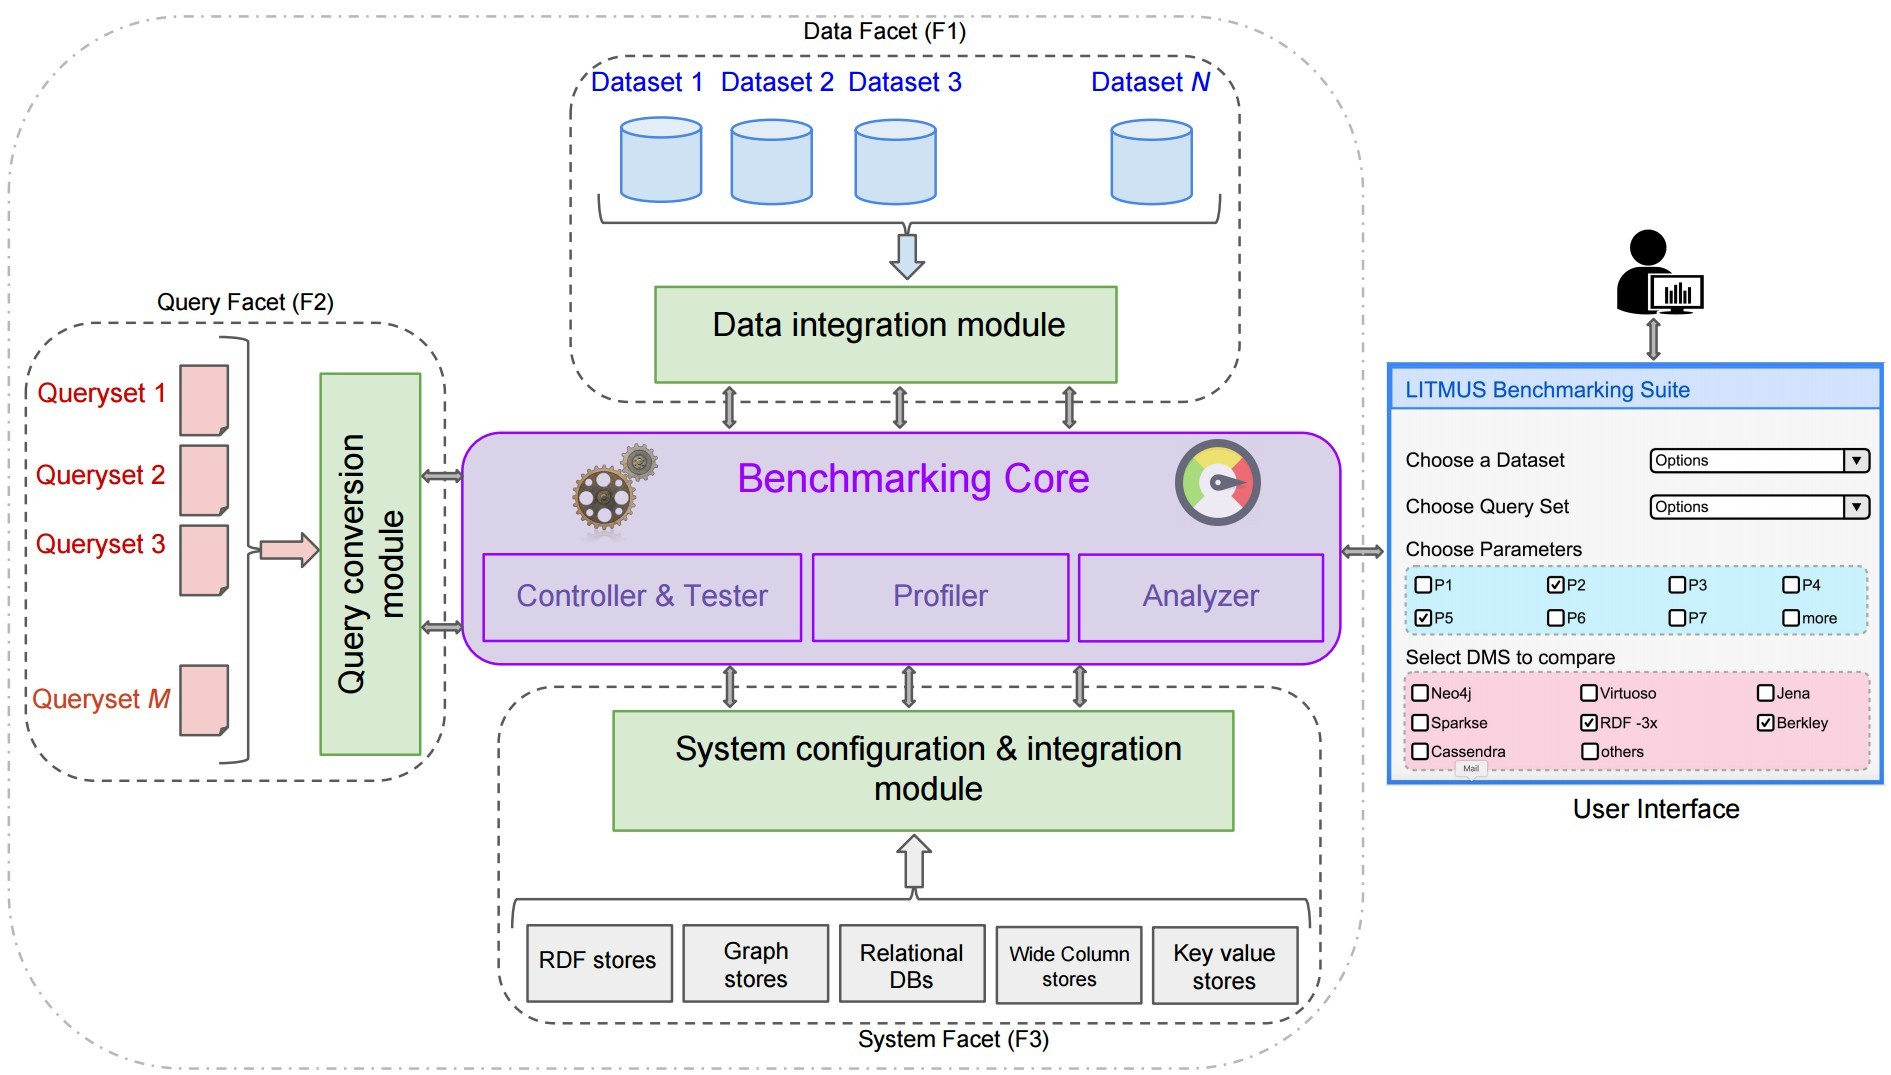
\includegraphics[scale=0.18]{images/benchmark_arch_latest_new}
            \caption{Overview of the LITMUS framework architecture.}
            \label{fig:benchmark_arch}
        \end{figure}
        
        \textbf{Data Facet \framebox[1.1\width]{F1}:} The Data Facet consists of two modules, \textit{(i)} Dataset(s) and \textit{(ii)} Data Integration Module. The \textit{dataset(s)} are the datasets chosen for benchmarking. These may be real datasets such as DBpedia\footnote{http://wiki.dbpedia.org/} Wikidata,\footnote{https://www.wikidata.org}; synthetic datasets such as the Berlin SPARQL Benchmarking (BSBM)~\cite{Bizer2009TheBS}, Waterloo SPARQL Diversity Test Suite (WatDiv)~\cite{alucc2014diversified}, or hybrid datasets which comprise both real and synthetic data. 
        The \textit{Data Integration Module} is responsible for (a) making the data available to the system in requested formats (such as .NT, CSV, SQL, JSON) by carrying out appropriate data conversion and mapping tasks (i.e. Challenge \textbf{C1}), and (b) loading the desired format of data to the respective DMSs selected for the benchmark. 
        
        \textbf{Query Facet \framebox[1.1\width]{F2}:} The Query Facet consists of two modules. (i) Queryset(s), and (ii) the Query Conversion Module. The \textit{Queryset} refers to the set of query input files. The \textit{Query Conversion Module} will be one of the key components addressing the language barrier (Challenge \textbf{C2}). This module is responsible for converting the input SPARQL queries to respective DMSs query language (for instance, SQL, CYPHER, CQL, etc). The conversion will be performed by developing an intermediate language/logic representation of the input query. The aim of this module is to allow efficient conversion of a wide variety of SPARQL queries (such as path, star-shaped and snowflake queries) to other respective query languages, ultimately solving the language barrier.
        
        \textbf{System Facet \framebox[1.1\width]{F3}:} The System Facet also consists of two key modules, (i) DMSs and (ii) DMS Configuration and Integration module. The \textit{DMSs} module  constitutes of the DMS selected for the benchmark. The \textit{DMS Configuration and Integration} module is responsible for (i) providing easy integration via wrapper(s) or as a plugin of the DMS to the end user, (ii) Monitor and configure the the integrated DMS for the benchmark. On top of this, this module will make use \textit{dockers} for ensuring a fair allocation of resources and necessary isolation required for conducting realistic benchmarks. 
        
        \textbf{Benchmarking core \framebox[1.1\width]{F4}:} The Benchmarking core (aka LITMUS core) is the heart of the LITMUS framework, consisting of three modules (i) Controller and Tester, (ii) Profiler, and (iii) Analyser. The \textit{Controller and Tester} is responsible for executing the respective scripts for: loading the data and queries to their corresponding DMSs, creating and validating the specified system configurations, and finally executing the benchmark on the selected setting. The \textit{Profiler} is responsible for: (a) generation and loading of various profiles (stress loads, query variations, etc) for conducting the benchmark tests and (b) writing the benchmark results profile-wise to the files (disk). The \textit{Analyser} is responsible for the collection of the results of the benchmark from the \textit{Profiler} and generates the performance evaluation reports. It also carries out the correlation analysis between the aforementioned  parameters by the user. The final results (reports) are then presented to the end user in a suitable visualization format.
        
\section{Conclusions} 
LITMUS addresses the gaps of the cross-benchmarking platform for different query languages and corresponding data management solutions. 
The literature review confirms the absence of such a (/proposed)  benchmarking platform under a single umbrella. 
We have (clearly) mentioned the upcoming challenges within the proposed system.
The empirical architecture of LITMUS proposes solutions to these challenges and would guide to achieve its objective.

\textbf{Acknowledgements}: Parts of this work are supported by funding received from the European Union's Horizon 2020 research and innovation program under the Marie Sklodowska-Curie grant agreement No 642795 (WDAqua ITN) and also from the EU H2020 Framework Programme provided for the projects Big Data Europe (GA no. 644564) and HOBBIT (GA no. 688227).

\bibliographystyle{abbrv}
\bibliography{ref}

\end{document}

